%!TEX root = ../sig-alternate.tex
\section{Petition analysis}
\label{sec:petition_analysis}

Given the list of petitions corresponding to campaigns on environmental issues on Twitter (described above), we first present an analysis on the petitions usage within different types of public campaigns and then analyze petition success by its visibility on Twitter.
%Finally, we propose a model to classify success of a particular campaign petition on Twitter.

\subsection{Petitions and tweets stats}
% * Number with petitions tweet stats: number of tweets; number of urls; number of valid urls with petitions;
Table~\ref{tab:petition_tweets} includes the basic figures extracted from our list of petitions\footnote{Latest petition signatures reassessment was on 28 Jan 2016.}.
Surprisingly, we notice that failed petitions aimed to gather only about half as much signatures as successful campaigns.
Furthermore, in our data, about a quarter of the petitions were successful, as opposed to only 1\% as found by~\citeauthor{Huang2015} \shortcite{Huang2015} across a broader range of petitions.
Overall, the tweets corresponding to the successful petitions are more likely to be passed on, i.e., they are retweeted about 4 times more frequently.

After a deeper inspection of the petition collection, we identified that over 6\% of the petitions in our dataset have a low signature goal $S(p)$, i.e., under 1,000 required signatures, out of which 13\% are identified as successful (as they reach their goal).
On the other hand, around 50\% of the petitions have a high initial goal (over 30,000) among which 35\% are successful.
Additionally, we observed that 39 petitions reached over 100K signatures while 130 petitions collected over 10K signatures.
The distribution of collected signatures is shown in Figure~\ref{fig:signatures_vs_rank}; it follows a Zipf distribution.

\begin{table}[hbt!]
\centering
\begin{tabular}{lccc}
			& \textit{Successful} & \textit{Failed}	\\ \midrule
Petitions					& 61		& 179		\\
Original tweets				& 601		& 716		\\
Original tweets users 		& 245		& 313		\\
Retweets						& 4828		& 1451 		\\
Retweets users				& 3965		& 1207		\\
Median $S(p)$				& 50000		& 15000		\\
Median $C(p)$				& 62997		& 6226		\\
\multicolumn{3}{l}{\textit{Petition tweets without campaign hashtags}}	\\ \midrule
Tweets						& 1054		& 707		\\
Users 						& 626		& 472		\\
\end{tabular}
\caption{Global statistics of the petition dataset of environmental campaigns. We show the data for the successful and failed petitions, as well as total numbers. Users are unique individuals who tweeted the petition URLs at least once. $S(p)$ and $C(p)$\footnote{Standard deviation for both $S(p)$ and $C(p)$ is within 270K} for successful and failed petitions are highlighted in the table. Additionally, we show statistics of the petition tweets that do not have a campaign hashtag.}
\label{tab:petition_tweets}
\end{table}

\begin{figure}
\centering
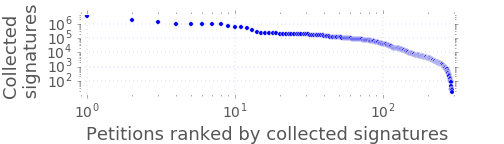
\includegraphics[width=\columnwidth]{figures/petitionsVSrank.png}
\caption{The final number of signatures received by each petition. The red line indicates the required number of signatures. A change in the slope of the zipf distribution occurs at 1K signatures, which represents a threshold for a petition to make a potential impact.}
\label{fig:signatures_vs_rank}
\end{figure}

\subsection{Petitions in public campaigns on Twitter}
% Information regarding environmental campaigns, types etc.
% Our findings:
% (a) only mobilization and single awareness; annual campaign with big number of msgs and failure rate.
% (b) doimated by the ever-growing campaigns.
% (c) Interesting examples (http://www.petitions.moveon.org/sign/legalize-hemp-farming/ - askdrh;
% https://you.38degrees.org.uk/petitions/stop-the-fracking-cover-up-by-defra - talkfracking (fracking censorship to delete.))

The following subsection provides answers for \textbf{RQ1} based on our analysis.
With only two exceptions, all the petitions were promoted through mobilization campaigns. The two exceptions are ``\#talkfracking'' and ``\#worldlovefordolphins'', which are both awareness campaigns.
Interestingly, these petitions with public campaigns hashtags were directed towards long-term plans, e.g., preventing ``covering up'' hydraulic fracturing by some organizations, or legalizing hemp farming.

As described in the Data Collection section, the campaign corpus is also annotated according to user engagement patterns for each campaign, and consists of four main types: one-day, ever-growing, annual, inactive.
We found that ``ever-growing'' campaigns (``\#saveafricananimals'', ``\#tweet4dolphins'' etc.) are the most active at tweeting about the petitions.
The rest $\sim$15\% of the campaigns are mainly ``inactive'' (``\#savethereef'', ``\#votegreen2015'').
Not surprisingly, ``one-day'' campaigns do not use petitions as their instruments given the very short timespans of such campaings.
Among campaigns with petitions, we also identified one ``annual'' campaign (``\#worldlovefordolphinsday'') that is advertising multiple ``Protect Dolphins'' petitions that tend to have a high failure rate.
Overall, there is no clear distinction between campaigns in terms of having dominantly successful petitions.
However, mobilization and ``ever-growing'' campaigns were the most active with petitions on Twitter.

\subsection{Campaign petitions on Twitter}
After data collection, cleaning and preprocessing, we extracted a number of features from the tweets containing a petition URL.
This process is explained in Section~\ref{sec:dataset} in detail.
To answer \textbf{RQ2}, we built a binary decision tree classifier\footnote{ http://scikit-learn.org } over our petition tweets collection using our set of features.

On average, the resulting tree has a relatively high branching factor, however a few paths are better at predicting the petition success.
We observe that the higher the signature goal, $S(p)$, of a particular petition, the more likely it is to succeed.
In particular, for the signature goal between between 100K and 300K 88\% of the petitions were successful.
However, setting a high petition goal may not guarantee its success. Success might also be correlated with various external factors, i.e., problem that a petition tries to address, external promotion (Facebook etc.), location of the petition owner etc.
Hence, the success factors for those campaigns are very different from the success factors of Kickstarter campaigns, for which failed campaigns have goals (amount of money) about three times higher than successful campaigns~\citeauthor{Etter2013} \shortcite{Etter2013}.

In our case, over 92\% of the petitions with $S(p)$ higher than 100K obtained their required number of signatures.
% TODO: Add some motivation, examples etc...
Regarding $T_3(p)$, the lower the average number of followers a campaign activist has, the less likely the petition is to attain the required number of signatures.
Similarly, the higher the average number of followers a user posting the petition URL without campaign hashtags has, the more likely the petition is to attain the required number of signatures.
We observe that the average number of followers is 10x higher for users outside of the campaign compared to campaign activists. 

\paragraph{Further Insights Towards RQ2}
Since it is not trivial to provide step-by-step instructions on how to drive your petition towards success in general, we would like to highlight some additional key points from our analysis.

% \pcm{I like the two following points; perhaps those should be the questions you pose in the introduction (research questions); then you could explicitly say that you come back to those questions here}

\textbf{Does petition success correlate with the number of tweets? - Yes.} We observed uniform distribution for the petitions with 0 tweets found on \textit{backtweets.com} in terms of $SignatureRate$. On the contrary, for the petitions with several tweets carrying its direct URL, $T_2(p)$, we observed a very high fraction of successful petitions (88\%). Pearson correlation for petitions with multiple tweets is 0.64 with \(p < 0.05\). This effect is particularly strong when we consider only retweets or tweets without campaign hashtags, $T_4(p)$. We observed similar behavior for \textit{thepetitionsite.com}.

\textbf{Does the number of users posting about the petition affect its success? - Yes.} We binned the petitions from the campaign corpus based on the $SignatureRate$, and extracted the average number of unique users posting about the petition in each bin. Figure~\ref{fig:signatures_vs_users} shows a boxer plot with the 25th, 50th and 75th percentiles for each bin. As a result, Pearson correlation is over 0.7 with \(p < 0.003\).

\begin{figure}
\centering
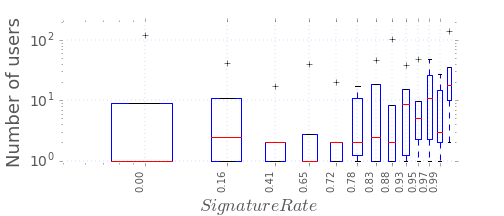
\includegraphics[width=\columnwidth]{figures/signaturesgoalVSnumusersCampaigns.png}
\caption{$SignatureRate$ against number of unique users posting about a petition on Twitter.}
\label{fig:signatures_vs_users}
\end{figure}

\textbf{Is it common to post (a) identical tweets without acknowledging original tweets or (b) retweet? - Retweet.} In our petition dataset we did not identify any duplicated tweets, i.e., tweets that are identical. Moreover, as shown in Table~\ref{tab:petition_tweets}, the number of retweets for the successful petitions is several times higher than the corresponding number for the unsuccessful ones.

\textbf{Which word features are more representative for tweets with successful petitions? - Uppercased.} We discovered that tweets with successful petitions have more words and uppercased words on average, by 9\% and 12\% respectively. We compared the distribution of the uppercased words between the collections of successful and failed petitions by computing the relative change for each word. We define it as follows: $RelativeChange = \frac{W_{succ} - W_{fail}}{W_{fail}}$, where $W_{succ}$ and $W_{succ}$ are the term frequencies of uppercased word $W$ for tweets with successful and failed petition. The top words from the successful collection are: ``ACTION'', ``URGENT'', ``WAZA'', ``PETITION'', ``SIGN'', while the unsuccessful petitions did not uppercase those words at all.
